\epigraph{The Babel fish is small, yellow, leech-like, and probably the oddest
thing in the universe. 
%It feeds on brainwave energy  ...
%absorbing all unconscious
%frequencies and then excreting telepathically a matrix formed from the conscious
%frequencies and nerve signals picked up from the speech centres of the brain,
%the practical upshot of which is that 
If you stick a Babel fish in your ear, you can
instantly understand anything in any form of language.}{{\it The Hitchhiker's
Guide to the Galaxy}. Douglas Adams.}
Human languages are diverse %and rich in categories 
with about 6000 to 7000
languages spoken worldwide \cite{languages}.
As civilization advances, the need for seamless communication and understanding across
languages becomes more and more crucial. Machine translation (MT), the
task of teaching machines to learn to translate automatically across languages, as
a result, is an important research area.
MT has a long history \cite{hutchins07} from the original
phiosophical ideas of universal languages in the $17^{\text{th}}$ century to
%first practical instances of MT in the twentieth century, e.g., one proposal by \newcite{weaver49}. 
\edit{
those first practical suggestions in the 1950s, most notably an influential %important
proposal by \newcite{weaver49} which marked the beginnings of MT research in
the United States. In that memorandum, Warren Weaver touched on
the idea of using computers to translate, specifically addressing the language
ambiguity problem by combining his knowledge of statistics,
cryptography, information theory, as well as logical and linguistic universals
\cite{hutchins2000early}.
Since then, MT has gone through many
periods of great development but also encountered several stagnant phases as
illustrated in \figref{f:mt_progress}.
Despite several moments of excitement that led to hopes that MT
will be solved ``very soon'' such as the 701 translator \cite{ibm701}
developed by scientists at Georgetown and IBM in the 1950s and the popular Google Translate
%or a simple vector-space transformation
%technique \cite{vectorspace} proposed by Google researchers 
at the beginning of the $21^{\text{st}}$ century \cite{brants07},
MT remains an extremely challenging problem \cite{solvemt,winograd_mt16}.
This motivates my work in the area of machine translation; specifically,
in this thesis, the goal is to advance neural machine translation (NMT), a new
promising approach for MT developed just recently, over the past two years. The results achieved in this
thesis on NMT together with work from other researchers have eventually
 produced a significant leap in the translation quality as illustrated in
\figref{f:mt_progress}. Before delving into details of the thesis, we now walk
the audience through the background and a bit of the development history of
machine translation.
}
%To understand why MT is difficult, let us trace through one ``evolution''
%path of % development
%MT which crosses through techniques that are used extensively in
%commercial MT systems. 

\begin{figure}[tbh!]
\centering
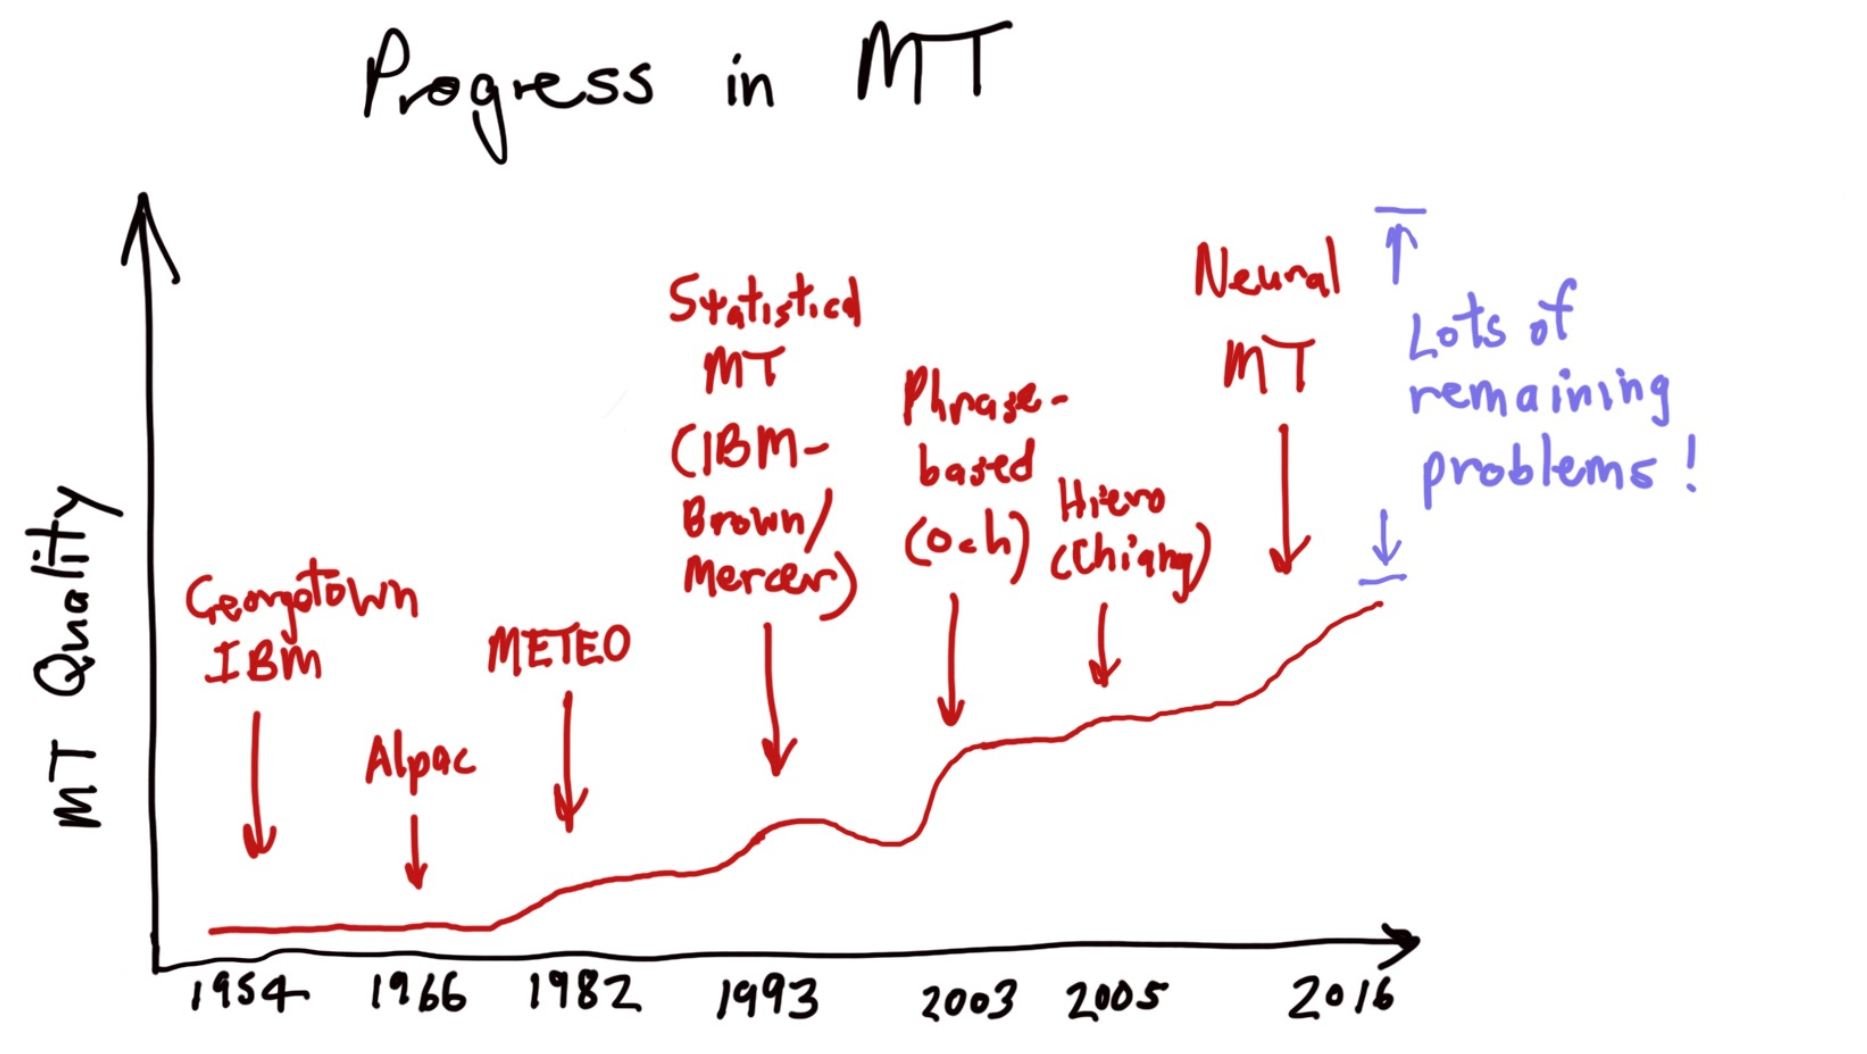
\includegraphics[width=\textwidth, clip=true, trim= 0 0 20 80]{img/MT_progress}
\caption[Machine translation progress]{{\bf Machine translation progress} --
from the 1950s, the starting of modern MT research, until the time of this
thesis, 2016, in which neural MT becomes a dominant approach. Image courtesy of
Christopher D. Manning.
} 
\label{f:mt_progress}
\end{figure}


\section{Machine Translation}
\label{sec:mt}
\begin{figure}
\centering
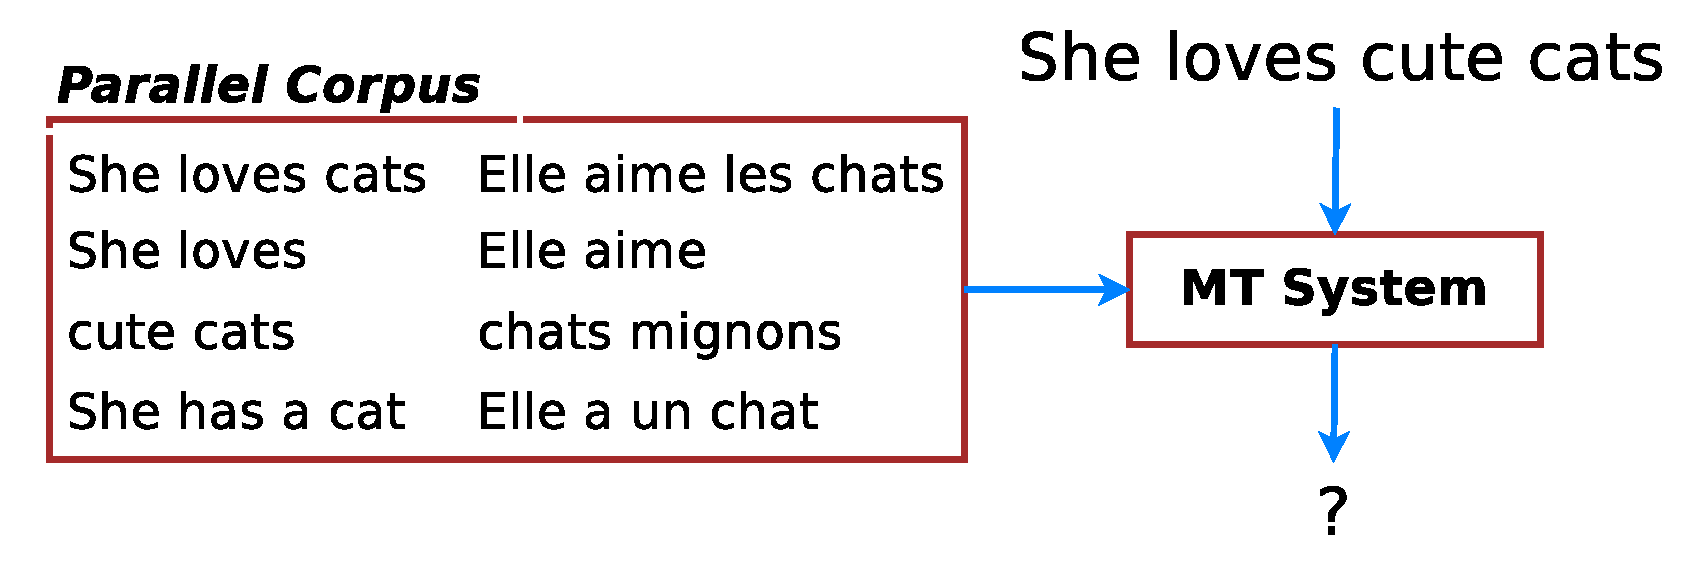
\includegraphics[width=\textwidth, clip=true, trim= 0 0 0 0]{img/mt.eps} % , angle=-90
\caption[Corpus-based approaches to machine translation]{{\bf Corpus-based approaches to
machine translation} -- a general setup in which MT systems
are built from parallel corpora of sentence pairs having the same meaning. Once
built, systems are used to translate new unseen
sentences, e.g., \word{She loves cute cats}.}
\label{f:mt}
\end{figure}

\edit{
Despite much enthusiasm, the beginning period of MT research in the 1950-60s,
was mostly about direct word-for-word replacement based on bilingual
dictionaries.\footnote{There are also proposals for ``interlingual'' and
``transfer'' approaches but these seemed to be too challenging to achieve, not
to mention limitations in hardware at that time\cite{hutchins07}.} An MT winner quickly came
right after the ALPAC report in 1966 pointing out that ``there is no immediate
or predictable prospect of useful machine translation'', which hampered MT
research for over a
decade. Fast-forwarding through the resurgence in the 1980s beginning with
Europe, Japan, and gradually the United States,
}
modern statistical MT started out with a seminal work by IBM scientists
\cite{Brown:1993:MSM}. The proposed {\it corpus-based} approaches require
minimal linguistic content and only need a {\it parallel} dataset of
sentence pairs which are translations of one
another, to train MT systems.
Such a language-independent setup is illustrated in Figure~\ref{f:mt}. 
\edit{
In more
detail, instead of hand building bilingual dictionaries which can be costly to
obtain, Brown and colleagues proposed to learn these dictionaries, or {\it
translation models}, probabilistically from parallel corpora. To accomplish
this, they propose a series of 5 algorithms of increasing complexity, often
referred as IBM Models 1-5, to learn {\it word alignment},
a mapping between source and target words in a parallel corpus, as illustrated
in \figref{f:wordalign}. The idea is
simple: the more often two words, e.g., \word{loves} and \word{aime}, occur
together in different sentence pairs, the more likely they are aligned to each
other and have equivalent meanings.
}

\begin{figure}[tbh!]
\centering
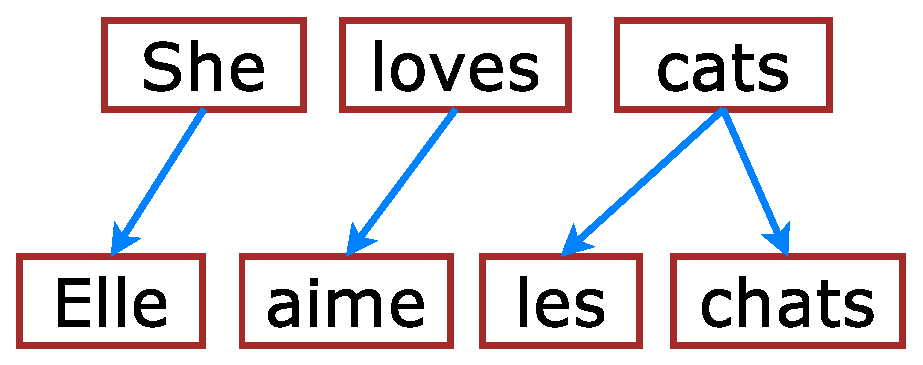
\includegraphics[width=0.35\textwidth, clip=true, trim= 0 0 0
0]{img/wordalign.eps}
\caption[Word-based alignment]{{\bf Word-based alignment} -- example of
an alignment between source and target words. In IBM
alignment models, each target word is aligned to at most one source word.
} 
\label{f:wordalign}
\end{figure}

\edit{
Once a translation model, i.e., a probabilistic bilingual dictionary, has been
learned, IBM model 1, the simplest and the most na\"{i}ve one among the five proposed
algorithms, translates a new source sentence as follows. First, it decides on
how long the translation is as well as how source words will be mapped to target
words as illustrated in Step 1 of \figref{f:wordmt_algo}. Then,
in Step 2, it produces a translation by selecting for each target position a
word that is the best translation for the aligned source word according to the
bilingual dictionary. Subsequent IBM models build on top of one another and refine the
translation story such as better modeling the reordering structure, i.e., how
word positions differ between source and target languages. We refer the audience to
the original IBM paper or Chapter 25 of \cite{Jurafsky:2009} for more details.
}
\begin{figure}[tbh!]
\centering
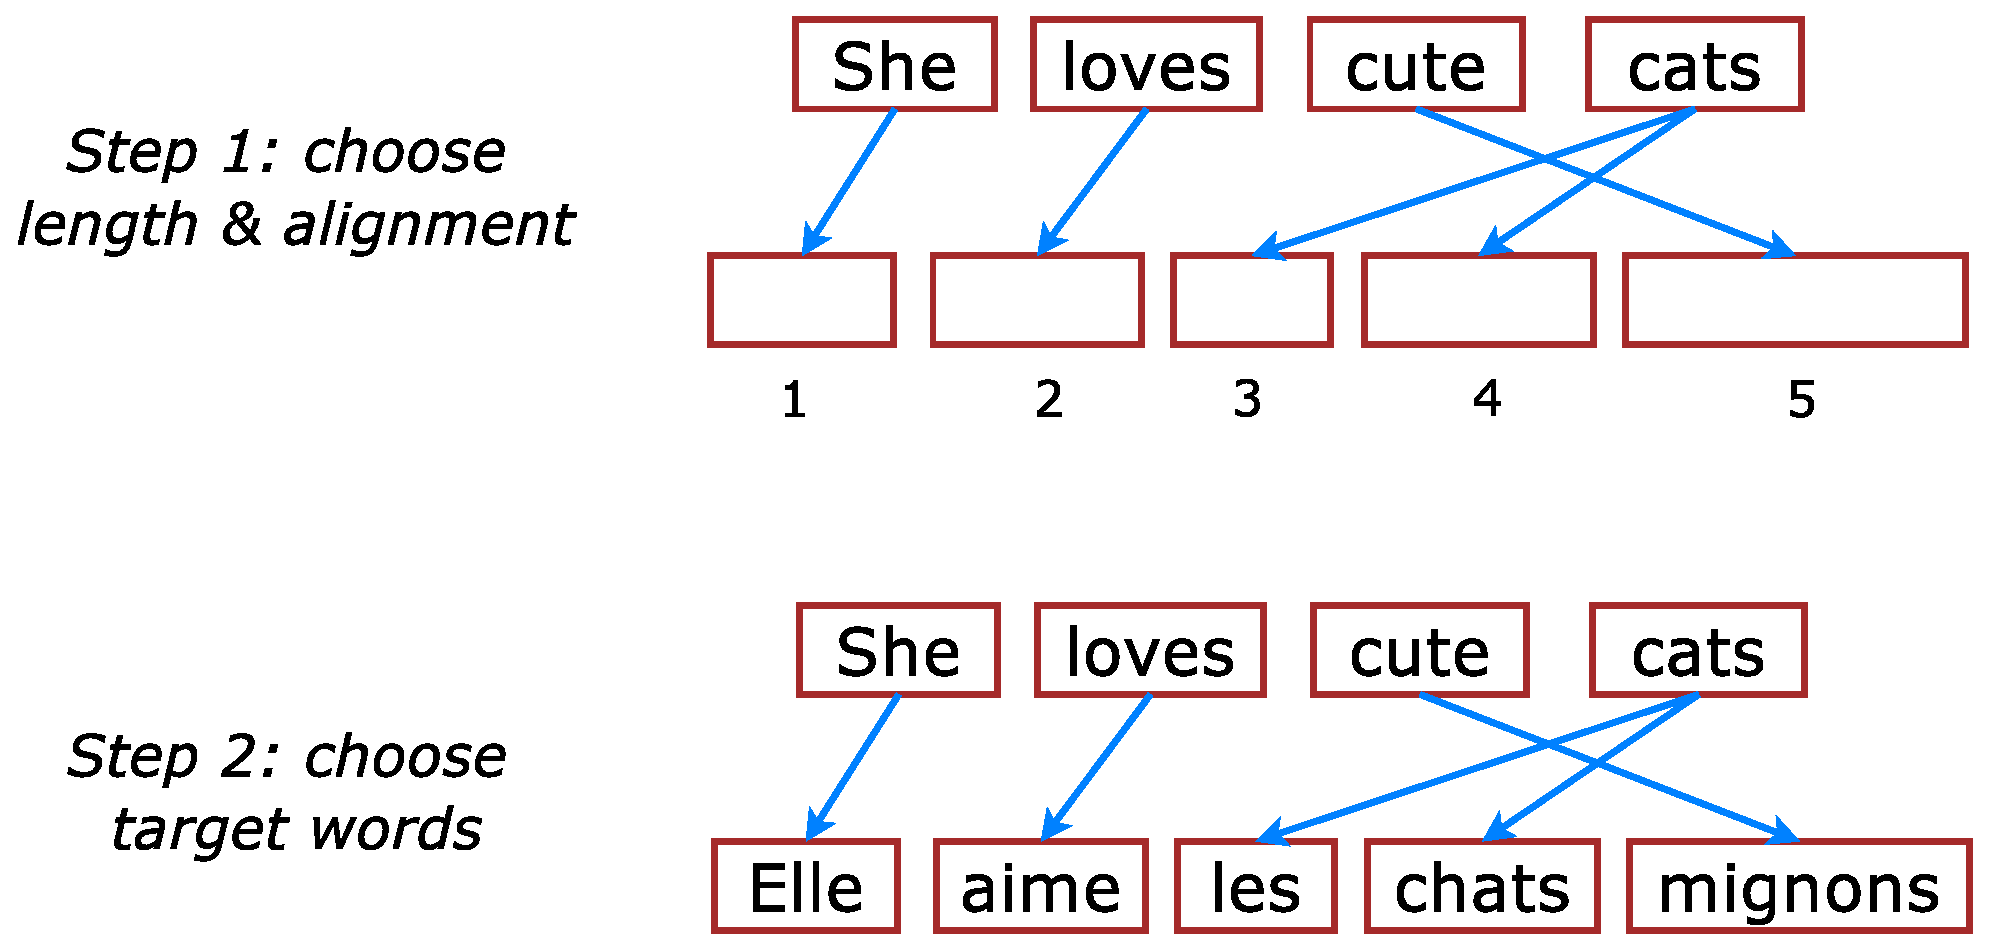
\includegraphics[width=0.8\textwidth, clip=true, trim= 0 0 0
0]{img/wordmt_algo.eps} % , angle=-90
\caption[A simple translation story]{{\bf A simple translation story} -- example of the generative story in
IBM Model 1 to produce a target translation given a source sentence and a
learned translation model.
} 
\label{f:wordmt_algo}
\end{figure}

\edit{
There are, however, two important details that we left out in the above translation story,
the {\it search} process and the {\it language modeling} component. In Step 1,
one might wonder among the exponentially many choices, how do we know what the
right translation length is and how source words should be mapped to target words? The
search procedure informally helps us ``browse'' through a manageable set of
candidates which are likely to include a good translation; whereas, the language
model will help us select the best translation among these candidates. We will
defer details of the search process to later since it is dependable on the
exact translation model being used. Language modeling, on the other hand, is an
important concept which has been studied earlier in speech recognition
\cite{katz87}. In a nutshell, a language model (LM)
learns from a corpus of monolingual text in the target language and collect
statistics on which sequence of words are likely to go with one another. When
applying to machine translation, an LM will assign high scores for coherent and
natural-sounding translations and low scores for bad ones.
For our example in the above figure, if the model happens to choose a wrong alignment, e.g.,
\word{cute} goes to position 3 while \word{cats} goes to positions 4 and 5, an
LM will alert us with a lower score given to that incorrect translation \word{Elle
aime mignons les chats} compared to the translation \word{Elle aime les chats
mignons} with a correct word ordering structure.\footnote{
\edit{
For completeness, translation and
language models are integrated together in an MT system through the {\it
Bayesian noisy channel} framework as follows:
\begin{align}
\label{e:noisy}
\hat{t} &= \argmax_t P(t|s) \approx \argmax_t P(s|t) P(t)
\end{align}
Here, we have a source sentence $s$ in which we ask our {\it decoder}, an
algorithm that implements the aforementioned search process, to find the best
translation, the $\argmax$ part. $P(s|t)$ represents the {\it translation} model, the
faithfulness of the translation in terms of meaning preservation between the source and the
target sentences; whereas $P(t)$
represents the {\it language} model, the fluency of the translated text.
}
}

While the IBM work had a huge impact on the field of statistical MT, researchers
quickly realized that word-based MT is insufficient as words
require context to properly translate, e.g., \word{bank} has two totally different
meanings when preceded by \word{financial} and \word{river}. As a result,
{\it phrase-based models}, \cite{Marcu:2002,Zens2002,Koehn:2003:SMT}, inter alia, became the de facto
standard in MT research and are still being the dominant approach in existing
commercial systems such as Google Translate until now. Much credit went to Och's
work on {\it alignment templates}, starting with his thesis in 1998 and later in
\cite{och03,och04}. The idea of alignment templates is to enable phrase-based MT
by first symmetrizing\footnote{\edit{Symmetrization is achieved by training IBM models
in both directions, source to target and vice versa, then intersecting the
alignments. There are subsequent techniques that jointly train alignments in
both directions such as \cite{liang06alignment}.}} the alignment to obtain many-to-many correspondences
between source and target words; in contrast, the original IBM models only produce
one-to-many alignments. From the symmetrized alignment, several heuristics have
been proposed to extract phrase pairs; the general idea is that phrase
pairs need to be ``consistent'' with their alignments: each word in a phrase
should not be aligned to a word outside of the other phrase. These pairs are stored
in what called a {\it phrase table} together with various scores to evaluate
phrase pairs in different aspects, e.g., how equivalent the meaning is, how good
the alignment is, etc. \figref{f:phrase_mt} gives an example of how a
phrase-based system translates.
}

\begin{figure}[tbh!]
\centering
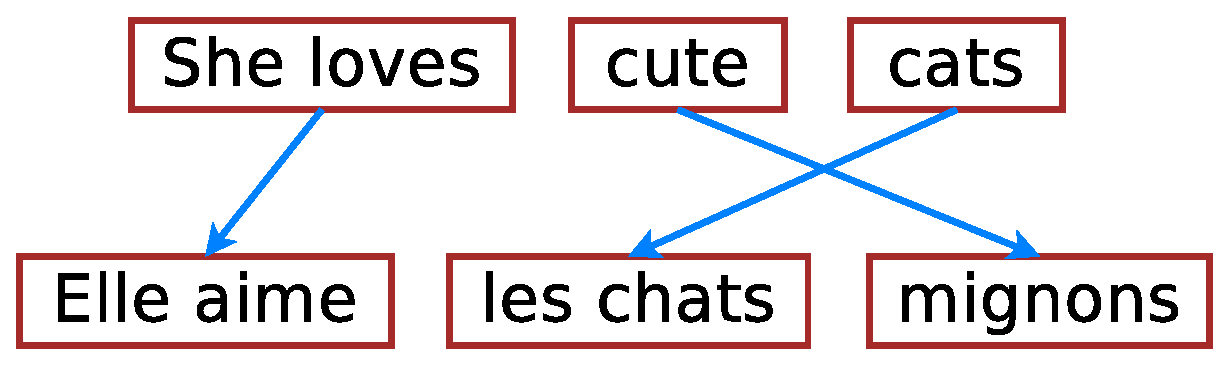
\includegraphics[width=0.45\textwidth, clip=true, trim= 0 0 0
0]{img/phrasemt.eps} % , angle=-90
\caption[Phrase-based machine translation]{{\bf Phrase-based machine translation} (MT) -- example of how phrase-based
MT systems translate a source sentence \word{She loves cute cats} into a target sentence
\word{Elle aime les chats mignons}: sentences are split into chunks and phrases
are translated.
} 
\label{f:phrase_mt}
\end{figure}

%% log-linear models %%
\edit{
State-of-the-art MT systems, in fact, contain more components than just the two
basic translation and language models. There are many knowledge
sources that can be useful to the translation task, e.g., language model,
translation model, reversed translation model, reordering
model\footnote{\edit{Reordering models learn the patterns of how words move across source
and target sentences and are trained based on the word alignment.}},
length/unknown penalties\footnote{\edit{To produce translations of appropriate lengths
and with a reasonable amount of unknown words, e.g., unseen names and numbers
at test time.}}, etc. To incorporate all of
these features, modern MT systems use a popular framework in natural language
processing, called the {\it maximum-entropy} or
{\it log-linear} model \cite{berger96,och02}, which has as its special case the
Bayesian noisy channel model that we briefly mentioned in \eq{e:noisy}.

Training log-linear MT models can be done using the standard {\it maximum
likelihood estimation} approach. However, in practice, these models are learned
by directly optimizing translation quality metrics such as BLEU
\cite{Papineni02bleu} in a technique known as {\it minimum error rate training}
or {\it MERT} \cite{och03mert}. Here, BLEU is an inexpensive automatic way of
evaluating the translation quality; the idea is to count words and phrases that
overlap between machine and human outputs. Despite many criticisms, BLEU is
still the most widely used evaluation metric up until now thanks to its
simplicity. 

Lastly, there has also been effort in
adding {\it syntax} to machine translation through tree-based models such as work by
\newcite{wu97,yamada01,chiang05}, inter alia. As illustrated in
\figref{f:mt_progress}, these approaches do provide gains
for several language pairs, mostly those that are significant different in terms
of sentence structures such as Chinese and English. However,
the gains are often modest compared to the added complexity of tree-based models
such as requirements to have good parsers and syntactic annotations.

For more information on evaluation metrics, tree-based models, and other
topics in statistical machine translation, we refer the audience to an 
excellent book by \newcite{koehn10smt}.
}


%remains to be the general approach for nowadays MT systems.
%For over twenty years since the IBM seminal paper, approaches in MT
%such as
%\cite{Koehn:2003:SMT,och03,Liang:2006:EDA,koehn2007moses,chiang07hiero,dyer10cdec,cer10phrasal},
%%inter alia, 
%are, by and large, similar according to the following two-stage
%process (see Figure~\ref{f:phrase_mt}). First, source sentences are broken into
%chunks which can be translated in isolation by looking up a ``dictionary'', or
%more formally a {\it translation model}. Translated target words and phrases
%are then put together to form coherent and natural-sounding sentences by consulting a
%{\it language model} (LM) on which sequences of words, i.e., {\it \ngram{}s}, are
%likely to go with one another.

\section{Neural Machine Translation}
%% interlingual idea, Vaquois diagram %%
%% briefly mention syntax-based %%

%The aforementioned approach
While statistical machine translation (SMT) has been successfully deployed in many
commercial systems, it does not work very well and suffers from the following
two major drawbacks.
First, translation decisions are {\it locally determined} as we translate
phrase-by-phrase and long-distance dependencies are often ignored. 
\edit{
More problematically, the entire MT pipeline is becoming increasingly {\it
complex} as more and more features are added to the log-linear framework
such as in recent MT systems \cite{galley08,chiang09,green13}. Many different
components need to be tuned
separately, e.g., translation models, language models, reordering models, etc.,
which makes it difficult to combine them together and to innovate. As a result,
the translation quality has saturated for SMT and big changes to the
existing framework were in dire need.

%Neural Machine Translation (NMT) is a new approach 
%to translating text from one
%language into another that captures long-range dependencies in sentences and
%generalizes better to unseen texts. The core of NMT is a single deep neural
%network with hundreds of millions of neurons that learn to directly map source
%sentences to target ones \cite{kal13,sutskever14,cho14}.
%NMT is appealing since it is conceptually
%simple and can be trained
%end-to-end. 
%Second, it is
%slightly unfortunate that language models (LMs), despite being a key component in the MT
%pipeline, utilize context information that is both short, consisting of only
%a handful of previous words, and target-only, never looking at the source
%words. These shortcomings in LMs gives rise to a new wave of {\it hybrid} systems which
%aim to empower phrase-based MT with neural network components, most notably
%\nlmtext{} (\nlms{}). 

Neural Machine Translation (NMT) is a new approach 
that addresses the aforementioned problems. First, NMT is a {\it single big neural
network} (with millions of artificial neurons) that is designed to model the
entire MT process 
% by learning to map source sentences to target ones 
\cite{kal13,sutskever14,cho14}. NMT requires {\it minimal domain knowledge}, just a
parallel corpus of source and target sentence pairs, similar to SMT, but with far
less preprocessing steps before a translation model can be built.
The most appealing feature of NMT is that it can be
trained {\it end-to-end} directly from the learning objective; hence, eliminating the
problem of having to learn multiple components in SMT systems. 

Unlike those intricate decoders (the search procedure we mentioned earlier) in popular SMT packages
\cite{koehn2007moses,chiang07hiero,dyer10cdec,cer10phrasal}, the translation
story of NMT is conceptually simple.
NMT translates as follows: an {\it encoder} reads through the given source
sentence to build a ``thought''
vector\footnote{This term was coined by Geoffrey Hinton in this article
\url{https://www.theguardian.com/science/2015/may/21/google-a-step-closer-to-developing-machines-with-human-like-intelligence}.},
a sequence of numbers that represents the sentence meaning; a {\it
decoder}, then, processes the sentence vector to emit a translation, as
illustrated in Figure~\ref{f:nmt}. 
This is often referred to as the encoder-decoder
architecture.\footnote{\edit{\newcite{allen87,chrisman91} wrote the very first papers
on %\newcite{forcada97} 
encoder-decoder models for translation!}} In this manner, NMT addresses the
local translation problem in SMT; it does not do phrase-by-phrase translation.
Instead, NMT gathers information from the entire source sentence before translating; as a result,
it can capture {\it long-range dependencies} in languages, e.g., gender
agreements; structural orderings of subject, verb, and object; etc.
\begin{figure}[tbh!]
\centering
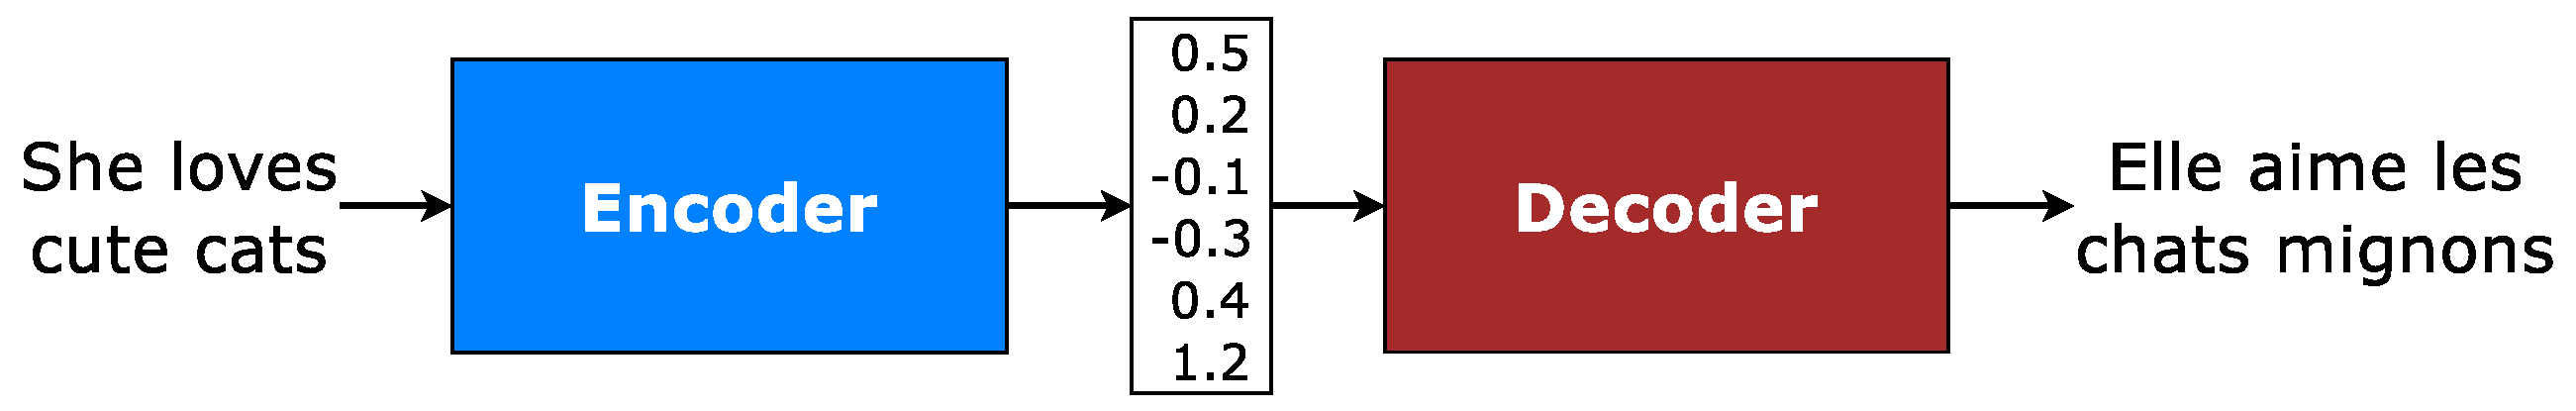
\includegraphics[width=\textwidth, clip=true, trim= 0 0 0 0]{img/encdec}
\caption[Encoder-decoder architecture]{{\bf Encoder-decoder architecture} --
example of the general approach for NMT. An {\it encoder} converts a source sentence
into a meaning vector which is passed through a {\it decoder} to produce a translation.
} 
\label{f:encdec}
\end{figure}

%Such simplicity leads to several advantages. 
%NMT requires minimal domain knowledge: it only assumes access to
%sequences of source and target words as training data and learns to directly
%map one into another. NMT beam-search decoders that
%generate words from left to right can be easily implemented, unlike the highly
%intricate decoders in standard MT \cite{Koehn:2003:SMT}. Lastly, the use of
%recurrent neural networks (RNNs) allow NMT to generalize well to very long word
%sequences while not having to 
%explicitly store any gigantic
%phrase tables or language models as in the case of standard MT.

A realization of NMT is to use a powerful model for sequential data, namely recurrent
neural network (RNN), for both the encoder and decoder \cite{sutskever14,cho14}.
Interested readers can find details about RNNs in
\secref{sec:rnn}; in a nutshell, RNNs allow us to build representations for
variable-length input -- in our case, sentences -- using a dynamic memory
structure. In \figref{f:nmt}, deep RNNs with two stacking layers are used to build
a sequence-based NMT: an encoder first constructs a representation for a source
sequence; a decoder, then, generates a target sequence,
one symbol at a time until a special end-of-sequence symbol is produced.

Sequence-based NMT has several advantages.
First, NMT beam-search decoders that generate words from left to right can be
easily implemented, unlike the highly complex beam-search decoders in SMT
\cite{Koehn:2003:SMT}. More importantly, the use of
RNNs allow NMT for {\it better generalization} to very long
sequences while not having to  explicitly store any gigantic
phrase tables or language models as in the case of SMT.
As sequence-based NMT is currently the de facto approach, we will use NMT to
generally refer to sequence-based NMT
throughout this thesis unless otherwise stated.

\begin{figure}[tbh!]
\centering
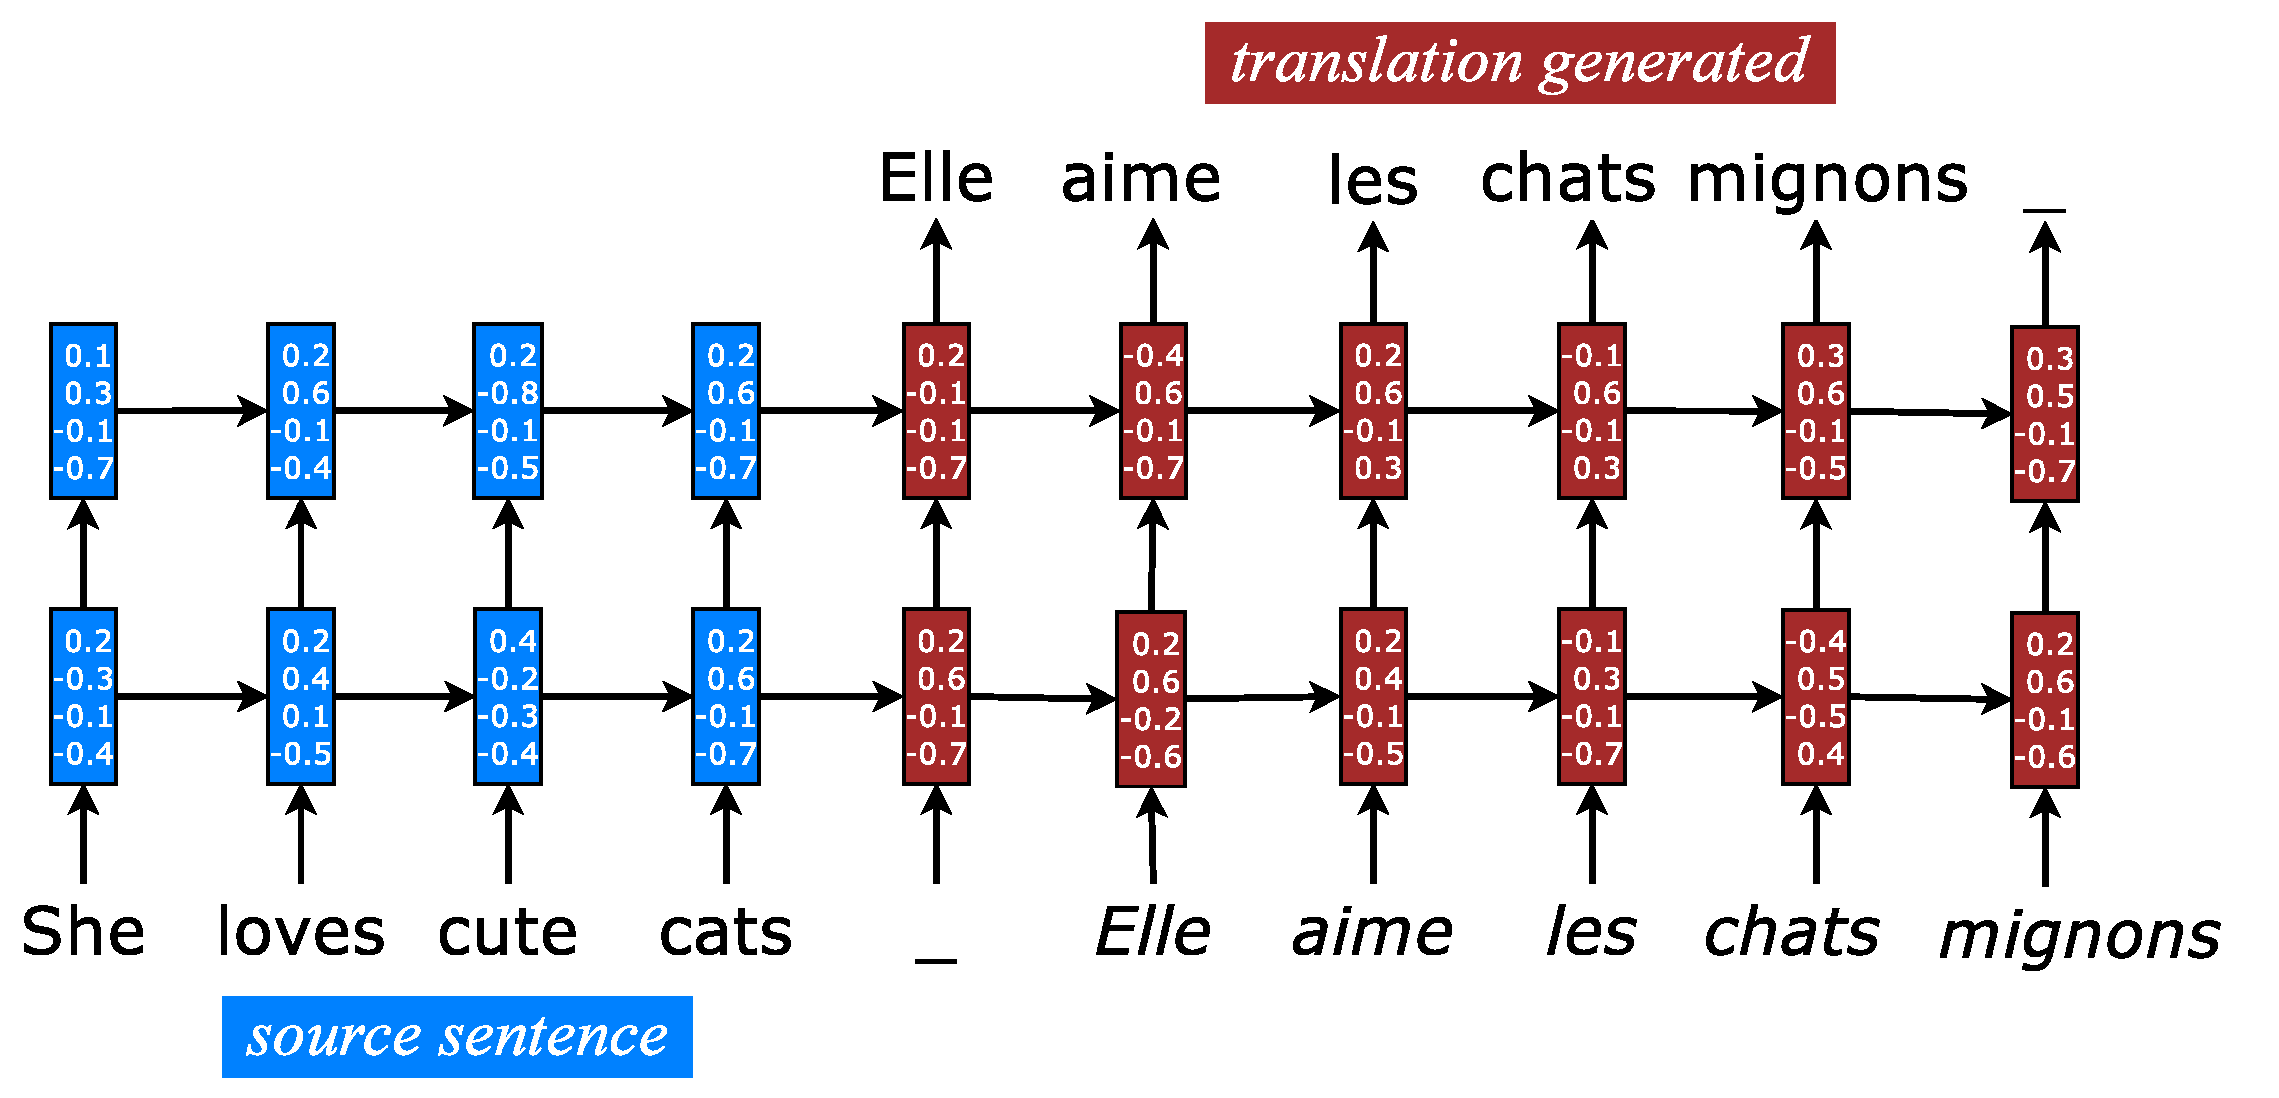
\includegraphics[width=\textwidth, clip=true, trim= 0 0 0
0]{img/nmt_intro} % , angle=-90
\caption[Sequence Models for NMT]{{\bf Sequence Models for NMT} -- example of a
deep recurrent architecture for translating a source sentence \word{She loves
cute cats} into a target sentence \word{Elle aime les chats mignons}. On the
decoder side, {\it words} generated from previous timesteps are used as inputs for the
next ones. Here, \word{\texttt{\_}} marks the end of a sentence.
} 
\label{f:nmt}
\end{figure}


%\begin{figure}[tbh!]
%\centering
%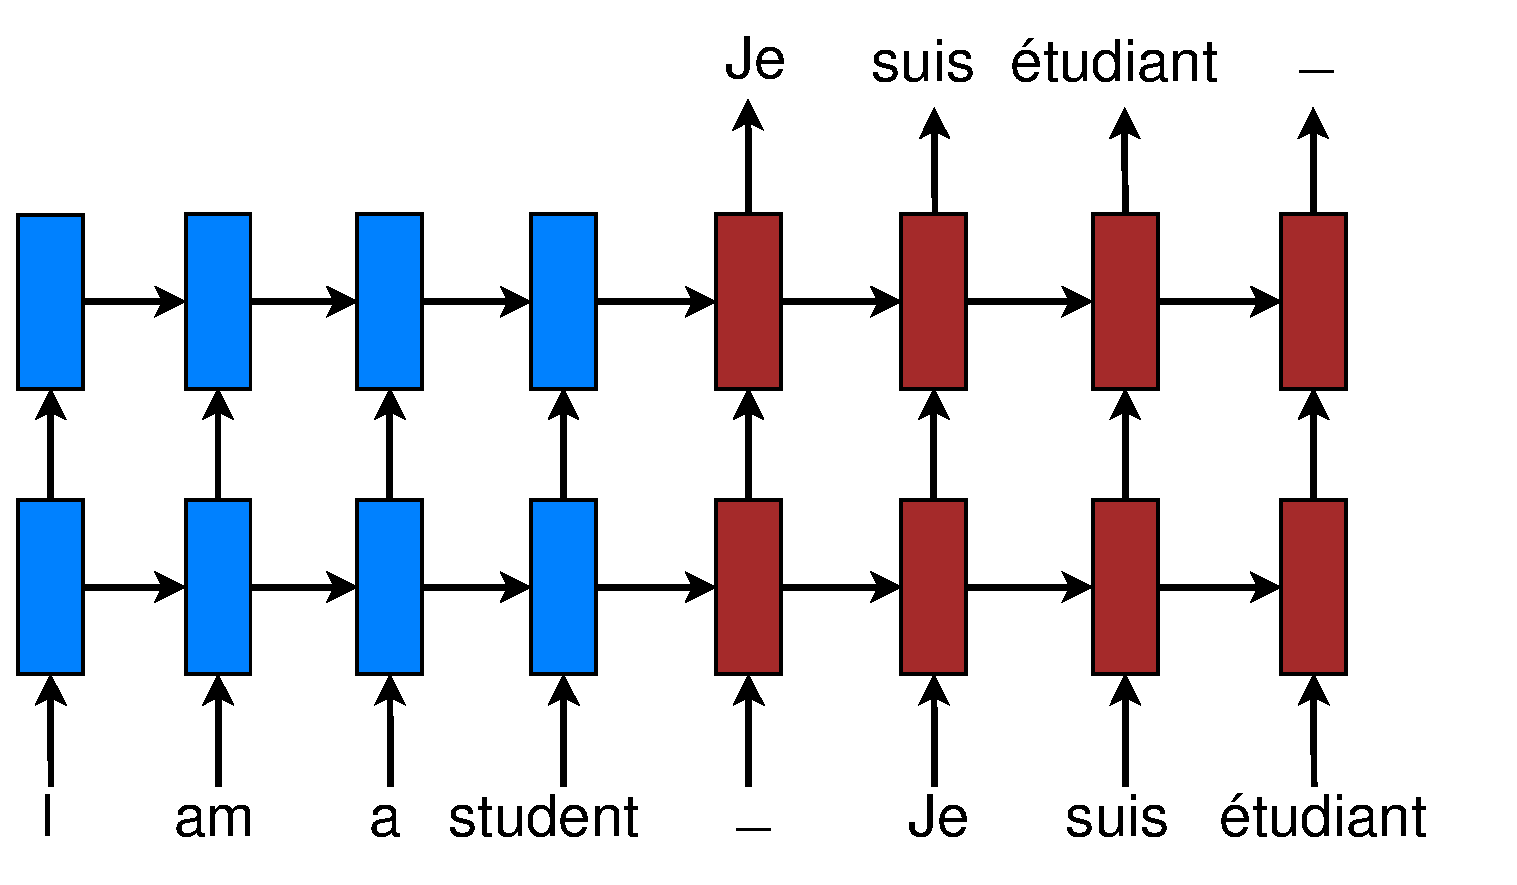
\includegraphics[width=\textwidth, clip=true, trim= 0 0 0
%0]{img/nmt_basic} % , angle=-90
%\caption[Neural machine translation]{{\bf Neural machine translation} -- example of a deep recurrent
%architecture proposed by \newcite{sutskever14} for
%translating a source sentence \word{I am a student} into a target sentence
%\word{Je suis \'{e}tudiant}. Here, \word{\texttt{\_}} marks the end of a sentence.
%} 
%\label{f:nmt}
%\end{figure}

}



\section{Thesis Outline}
Despite all the aforementioned advantages and potentials, the early NMT architecture
\cite{sutskever14,cho14} still has many drawbacks. In this thesis, I will
highlight three problems pertaining to the existing NMT model, namely the
{\it vocabulary coverage}, the {\it memory constraint}, and the {\it
language complexity} issues. Each chapter is devoted to solving one of these
problems. In each chapter, I will describe how I have pushed the limits of NMT, making it
applicable to a wide variety of languages with state-of-the-art performance such as
English-French \cite{luong15}, English-German \cite{luong15attn,luong15iwslt},
English-Vietnamese \cite{luong15iwslt}, and
English-Czech \cite{luong16}. Towards the {\it future} of
NMT, I answer two questions: (1) whether we can improve translation by jointly
learning from a wide variety of sequence-to-sequence tasks such as parsing,
image caption generation, and auto-encoders or skip-thought vectors
\cite{luong16iclr}; and (2)
whether we can compress NMT for mobile devices \cite{see16}.
In brief, this thesis is organized as follows. I start off by providing background knowledge on RNN and NMT
in Chapter~\ref{c:background}. 
The aforementioned three problems and approaches to the future of NMT are detailed in
Chapters~\ref{c:copy},~\ref{c:attention},~\ref{c:hybrid}, and~\ref{c:future}
respectively, which we will go through one by one next.
%My contributions are detailed in:
%Chapter~\ref{c:copy} on the rare word problem, Chapter~\ref{c:attention} on the
%sentence length problem, Chapter~\ref{c:hybrid} on the language complexity
%problem, and Chapter~\ref{c:future} on the future of NMT.
Chapter~\ref{c:conclude} wraps up and discusses remaining challenges in NMT research.

\subsubsection*{Copy Mechanisms} 
%\paragraph{Copy Mechanisms} 
A significant weakness in the first NMT 
systems is their inability to correctly translate very rare words:  
end-to-end NMTs tend to have relatively small vocabularies with a single
\unk{} symbol that represents every possible out-of-vocabulary (OOV) word. In
Chapter~\ref{c:copy}, I propose simple and effective techniques to address this
{\it vocabulary size} problem through teaching NMT to ``copy'' words from source to
target. Specifically, I train an NMT system on data that is augmented by the output of a word 
alignment algorithm, allowing the NMT system to emit, for each OOV word
in the target sentence, the position of its corresponding word in the source sentence.
This information is later utilized in a
post-processing step that translates every OOV word using a dictionary. My 
experiments on the WMT'14 English to French translation task show that this 
method provides a substantial improvement of up to 2.8 BLEU points over an
equivalent NMT system that does not use this technique. 
With 37.5 BLEU points, this NMT system is the first to surpass 
the best result achieved on a WMT'14 contest task. 
\edit{{\it This chapter is based
on the following paper \cite{luong15} in which I, Ilya Sutskever, and Quoc Le
share the first co-authorship.}}

\subsubsection{Attention Mechanisms} 
%\paragraph{Attention Mechanisms} 
While NMT can translate well for short- and medium-length sentences, it 
has a hard time dealing with long sentences.
An attentional mechanism was proposed by \newcite{bog15} to address that {\it
sentence length} problem by
selectively focusing on parts of the source sentence during translation. However,
there has been little work exploring useful architectures for attention-based
NMT. Chapter~\ref{c:attention} examines two simple and effective classes of attentional
mechanism: a {\it global} approach which always attends to all source words and
a {\it local} one that only looks at a subset of source words at a time. 
I demonstrate the effectiveness of both approaches on the WMT translation
tasks between English and German in both directions. With local
attention, I achieve a significant gain of 5.0 BLEU points over
non-attentional systems that 
already incorporate known techniques such as dropout. My ensemble 
model using different attention architectures yields a new
state-of-the-art result in the WMT'15 English to German
translation task with 25.9 BLEU points, an improvement of 1.0 BLEU points over the existing
best system backed by NMT and an $n$-gram reranker. 
\edit{{\it This chapter is based
on the following papers \cite{luong15attn,luong15iwslt}.}}
\error{Mention results from IWSLT, for TED talk English-German,
English-Vietnamese}

\subsubsection{Hybrid Models} 
%\paragraph{Hybrid Models} 
Nearly all previous NMT work has used quite restricted
vocabularies, perhaps with a subsequent method to patch in unknown words such as
the copy mechanisms mentioned earlier. While effective, the copy mechanims cannot deal with all the
complexity of human languages such as rich morphology, neologisms, and informal
spellings.
Chapter~\ref{c:hybrid} presents a novel word-character solution to that {\it
language complexity} problem towards achieving
open vocabulary NMT.
I build hybrid systems that translate mostly at the {\it word}
level and consult {\it character} components for rare words. 
My character-level recurrent neural networks compute source
word representations and recover unknown target words when needed.
The twofold advantage of such a hybrid approach is that it is much faster and easier to
train than character-based ones; at the same time, it never produces unknown words as in the case of word-based models. 
On the WMT'15 English to Czech translation task, 
this hybrid approach offers an addition boost of +$2.1{-}11.4$ BLEU points over models 
that already handle unknown words. 
My best system achieves a new state-of-the-art result with
$20.7$ BLEU score.
I demonstrate that my character models can successfully learn to not only generate well-formed words for Czech, a
highly-inflected language with a very complex vocabulary, but also build correct
representations for English source words.
\edit{{\it This chapter is based on the following paper \cite{luong16}.}}

\subsubsection{NMT Future} 
%\paragraph{NMT Future} 
Chapter~\ref{c:future} answers the two aforementioned questions
for the future of NMT: whether we can utilize other tasks to improve
translation and whether we can compress NMT models. 
\edit{
The former question is important because of the fact that the first NMT systems only
utilize parallel corpora despite an abundant amount of available data from
monolingual and multi-lingual corpora as well as data from related tasks. The
latter question is motivated by the indispensable role of mobile devices in nowadays
society\footnote{In 2014, the number of mobile devices is more than the number
of people in the world according to
\url{http://www.independent.co.uk/life-style/gadgets-and-tech/news/there-are-officially-more-mobile-devices-than-people-in-the-world-9780518.html}.}
and the fact that state-of-the-art NMT models are beyond the storage capacity of
existing mobile gadgets.
}

%, I answer two questions in Chapter~\ref{c:future}: (1) whether we can improve translation by jointly
%learning from a wide variety of sequence-to-sequence tasks such as parsing,
%image caption generation, and auto-encoders or skip-thought vectors; and (2)
%whether we can compress NMT for mobile devices.

For the first question, 
I examine three multi-task learning (MTL) settings for sequence to sequence
models:
(a) the {\it one-to-many} setting -- where the encoder is shared
between several tasks such as machine translation and
syntactic parsing, (b) the {\it many-to-one} setting -- useful when only the
decoder can be shared, as in the case of 
translation and image caption generation, and (c) the {\it
  many-to-many} setting -- where multiple encoders and decoders are
shared, which is the case with unsupervised objectives
and translation.  My results show that training on a small amount of parsing and
image caption data can improve the translation quality between English and
German by up to $1.5$ BLEU
points over strong single-task baselines on the WMT benchmarks. Rather
surprisingly,
I have established a new {\it
state-of-the-art} result in constituent parsing with 93.0 F$_1$ by utilizing
translation data. Lastly, I reveal interesting properties of the two unsupervised learning
objectives, autoencoder and skip-thought, in the MTL context: an autoencoder helps less in terms of
perplexity but more on BLEU scores compared to skip-thought.
\edit{{\it This section is based on the following paper \cite{luong16iclr}.}}

%Neural Machine Translation (NMT), like many other deep learning domains, typically suffers from over-parameterization, resulting in large storage sizes.
For the second question, I examine three simple magnitude-based pruning schemes to compress NMT models, namely {\it class-blind}, {\it class-uniform}, and {\it class-distribution}, which differ in terms of how pruning thresholds are computed for the different classes of weights in the NMT architecture.
I demonstrate the efficacy of weight pruning as a compression technique for a state-of-the-art NMT system. 
I show that an NMT model with over 200 million parameters can be pruned by 40\% with very little performance loss as measured on the WMT'14 English-German translation task. 
This sheds light on the distribution of redundancy in the NMT architecture.
My main result is that with {\it retraining}, I can recover and even surpass the original performance with an 80\%-pruned model. 
\edit{{\it This section is based on the following paper \cite{see16} in which
Abigail See and I share the first co-authorship.}}

\edit{
\subsubsection{Wrap-up} 
In summary, this thesis has touched on a variety of aspects in which NMT can be
significantly improved. My hope is to convince the audience 
at the end of this thesis that NMT models have successfully taken over the role
of SMT models and will continue to be the de factor standard for several years
to come. Still, there are many challenging and rewarding problems to be explored
which I will summarize in the conclusion chapter. {\it The material is based on an
NMT tutorial given by me, Kyunghuyn Cho, and Christopher D. Manning at
ACL'2016}.\footnote{The tutorial website is
\url{https://sites.google.com/site/acl16nmt/}.}
}

\error{
\subsubsection{Related publications}
\cite{luong13}

\cite{luong15nlm}
}
%We start off by providing background knowledge on RNN and NMT
%in Chapter~\ref{c:background}. The following chapters detail my contributions.
%Chapter~\ref{c:copy} discusses how the rare word
%problem in NMT is addressed with a mechanism to ``copy'' words from source to
%target; hence, extending the vocabulary
%coverage. Chapter~\ref{c:attention} describes
%how the attention mechanism, a way to select
%local contexts in the source sentence as we transate, can be effectively used in
%NMT to better handle long sentences. Chapter~\ref{c:hybrid} 
%proposes a novel way of dealing with language complexity (rich morphology,
%neologisms, and informal spellings) by building a hybrid word and character
%level model which can gain from the flexibility of a character-level model while
%maintaining the speed and quality of the word-level model. Towards the future of
%NMT, I answer two questions in Chapter~\ref{c:future}: (1) whether we can improve translation by jointly
%learning from a wide variety of sequence-to-sequence tasks such as parsing,
%image caption generation, and auto-encoders or skip-thought vectors; and (2)
%whether we can compress NMT for mobile devices.
%Chapter~\ref{c:conclude} wraps up and discusses remaining challenges in NMT
%research.


%Due to computational constraint, NMT has to limit its vocabulary to a fixed set
%of top frequent words, e.g., the top 50K words. As a result, all other words
%are represented by a universal symbol \unk{}.
%
%I discuss in Chapter~\ref{c:copy} discusses how the rare word
%problem in NMT is addressed with a mechanism to ``copy'' words from source to
%target; hence, extending the vocabulary
%coverage.

